\documentclass[a4paper,10pt]{article}
\usepackage[english]{babel}
\usepackage[utf8]{inputenc}

%
% Graphics
%
\usepackage{graphicx}
\usepackage{xcolor}

\definecolor{alpha}{HTML}{3FA9F5}

%
% Bibliography
%
\usepackage[backend=bibtex,maxnames=5,sorting=none,url=false]{biblatex}
\usepackage{csquotes}

%
% Listings
%
\usepackage{listings}

\definecolor{background}{HTML}{FAFAFA}
\definecolor{sign}{HTML}{3FA9F5}

\lstdefinelanguage{fortune}{
  basicstyle=\ttfamily,
  basewidth={0.5em,0.5em},
  backgroundcolor=\color{background},
  literate=
   *{\%}{{{\color{alpha}{\%}}}}{1}
}

\lstdefinelanguage{shell}{
  basicstyle=\ttfamily,
  basewidth={0.5em,0.5em},
  backgroundcolor=\color{background},
  literate=
    [*]{\\\$}{{{\color{alpha}{\$}}}}{1}
       {Command>}{{{\color{alpha}{Command>}}}}{8}
       {ivan(0)>}{{{\color{alpha}{ivan(0)>}}}}{8}
       {ivan(1)>}{{{\color{alpha}{ivan(1)>}}}}{8}
       {ivan(0):RELEASED>}{{{\color{alpha}{ivan(0):RELEASED>}}}}{17}
       {ivan(0):LOCKED>}{{{\color{alpha}{ivan(0):LOCKED>}}}}{15}
       {ivan(1):LOCKED>}{{{\color{alpha}{ivan(1):LOCKED>}}}}{15}
       {ivan(2):LOCKED>}{{{\color{alpha}{ivan(2):LOCKED>}}}}{15}
}

\lstdefinelanguage{json}{
  basicstyle=\ttfamily,
  basewidth={0.5em,0.5em},
  backgroundcolor=\color{background},
  literate=
   *{:}{{{\color{alpha}{:}}}}{1}
    {,}{{{\color{alpha}{,}}}}{1}
    {\{}{{{\color{alpha}{\{}}}}{1}
    {\}}{{{\color{alpha}{\}}}}}{1}
    {[}{{{\color{alpha}{[}}}}{1}
    {]}{{{\color{alpha}{]}}}}{1}
}

\lstnewenvironment{fortune}%
{\lstset{language=fortune}}%
{}

\lstnewenvironment{json}%
{\lstset{language=json}}%
{}

\lstnewenvironment{shell}%
{\lstset{language=shell}}%
{}

%
% Links
%
\usepackage{hyperref}
\hypersetup{%
  colorlinks=true,
  citecolor={alpha},
  linkcolor={alpha},
  urlcolor ={alpha}
}

%
% Text
%
\newcommand{\ie}{i.e.}
\newcommand{\eg}{e.g.}
\newcommand{\etc}{etc.}

\newcommand{\fix}{should be modified}
\newcommand{\leave}{no changes are needed}
\newcommand{\overwrite}{should contain your previous changes}

\newcommand{\python}{\texttt{Python}}
\newcommand{\classname}[1]{\texttt{#1}}
\newcommand{\filename}[1]{\texttt{#1}}
\newcommand{\code}[1]{\texttt{#1}}

%
% References
%
\newcommand{\sref}[1]{Section~\ref{sec:#1}}
\newcommand{\tref}[1]{Table~\ref{tab:#1}}
\newcommand{\fref}[1]{Figure~\ref{fig:#1}}

\newcommand{\slabel}[1]{\label{sec:#1}}
\newcommand{\tlabel}[1]{\label{tab:#1}}
\newcommand{\flabel}[1]{\label{fig:#1}}

\newcommand{\slab}[1]{\label{sec:#1}}
\newcommand{\tlab}[1]{\label{tab:#1}}
\newcommand{\flab}[1]{\label{fig:#1}}

\newcommand{\aref}[1]{Lab~#1 \cite{description#1}}


\bibliography{include/references.bib}

\title{%
  Distributed Systems: Lab 0\\%
  Standalone Database%
}
\author{Petru Eles and Adrian Horga\\
\vspace{0.5em}
\href{mailto:petru.eles@liu.se}{petru.eles@liu.se} and
\href{mailto:adrian.horga@liu.se}{adrian.horga@liu.se}
}
% \date{December 27, 2016}

\begin{document}
\maketitle

\section{Introduction to the Programming Project} \slab{data-format}
\begin{figure}
  \centering
  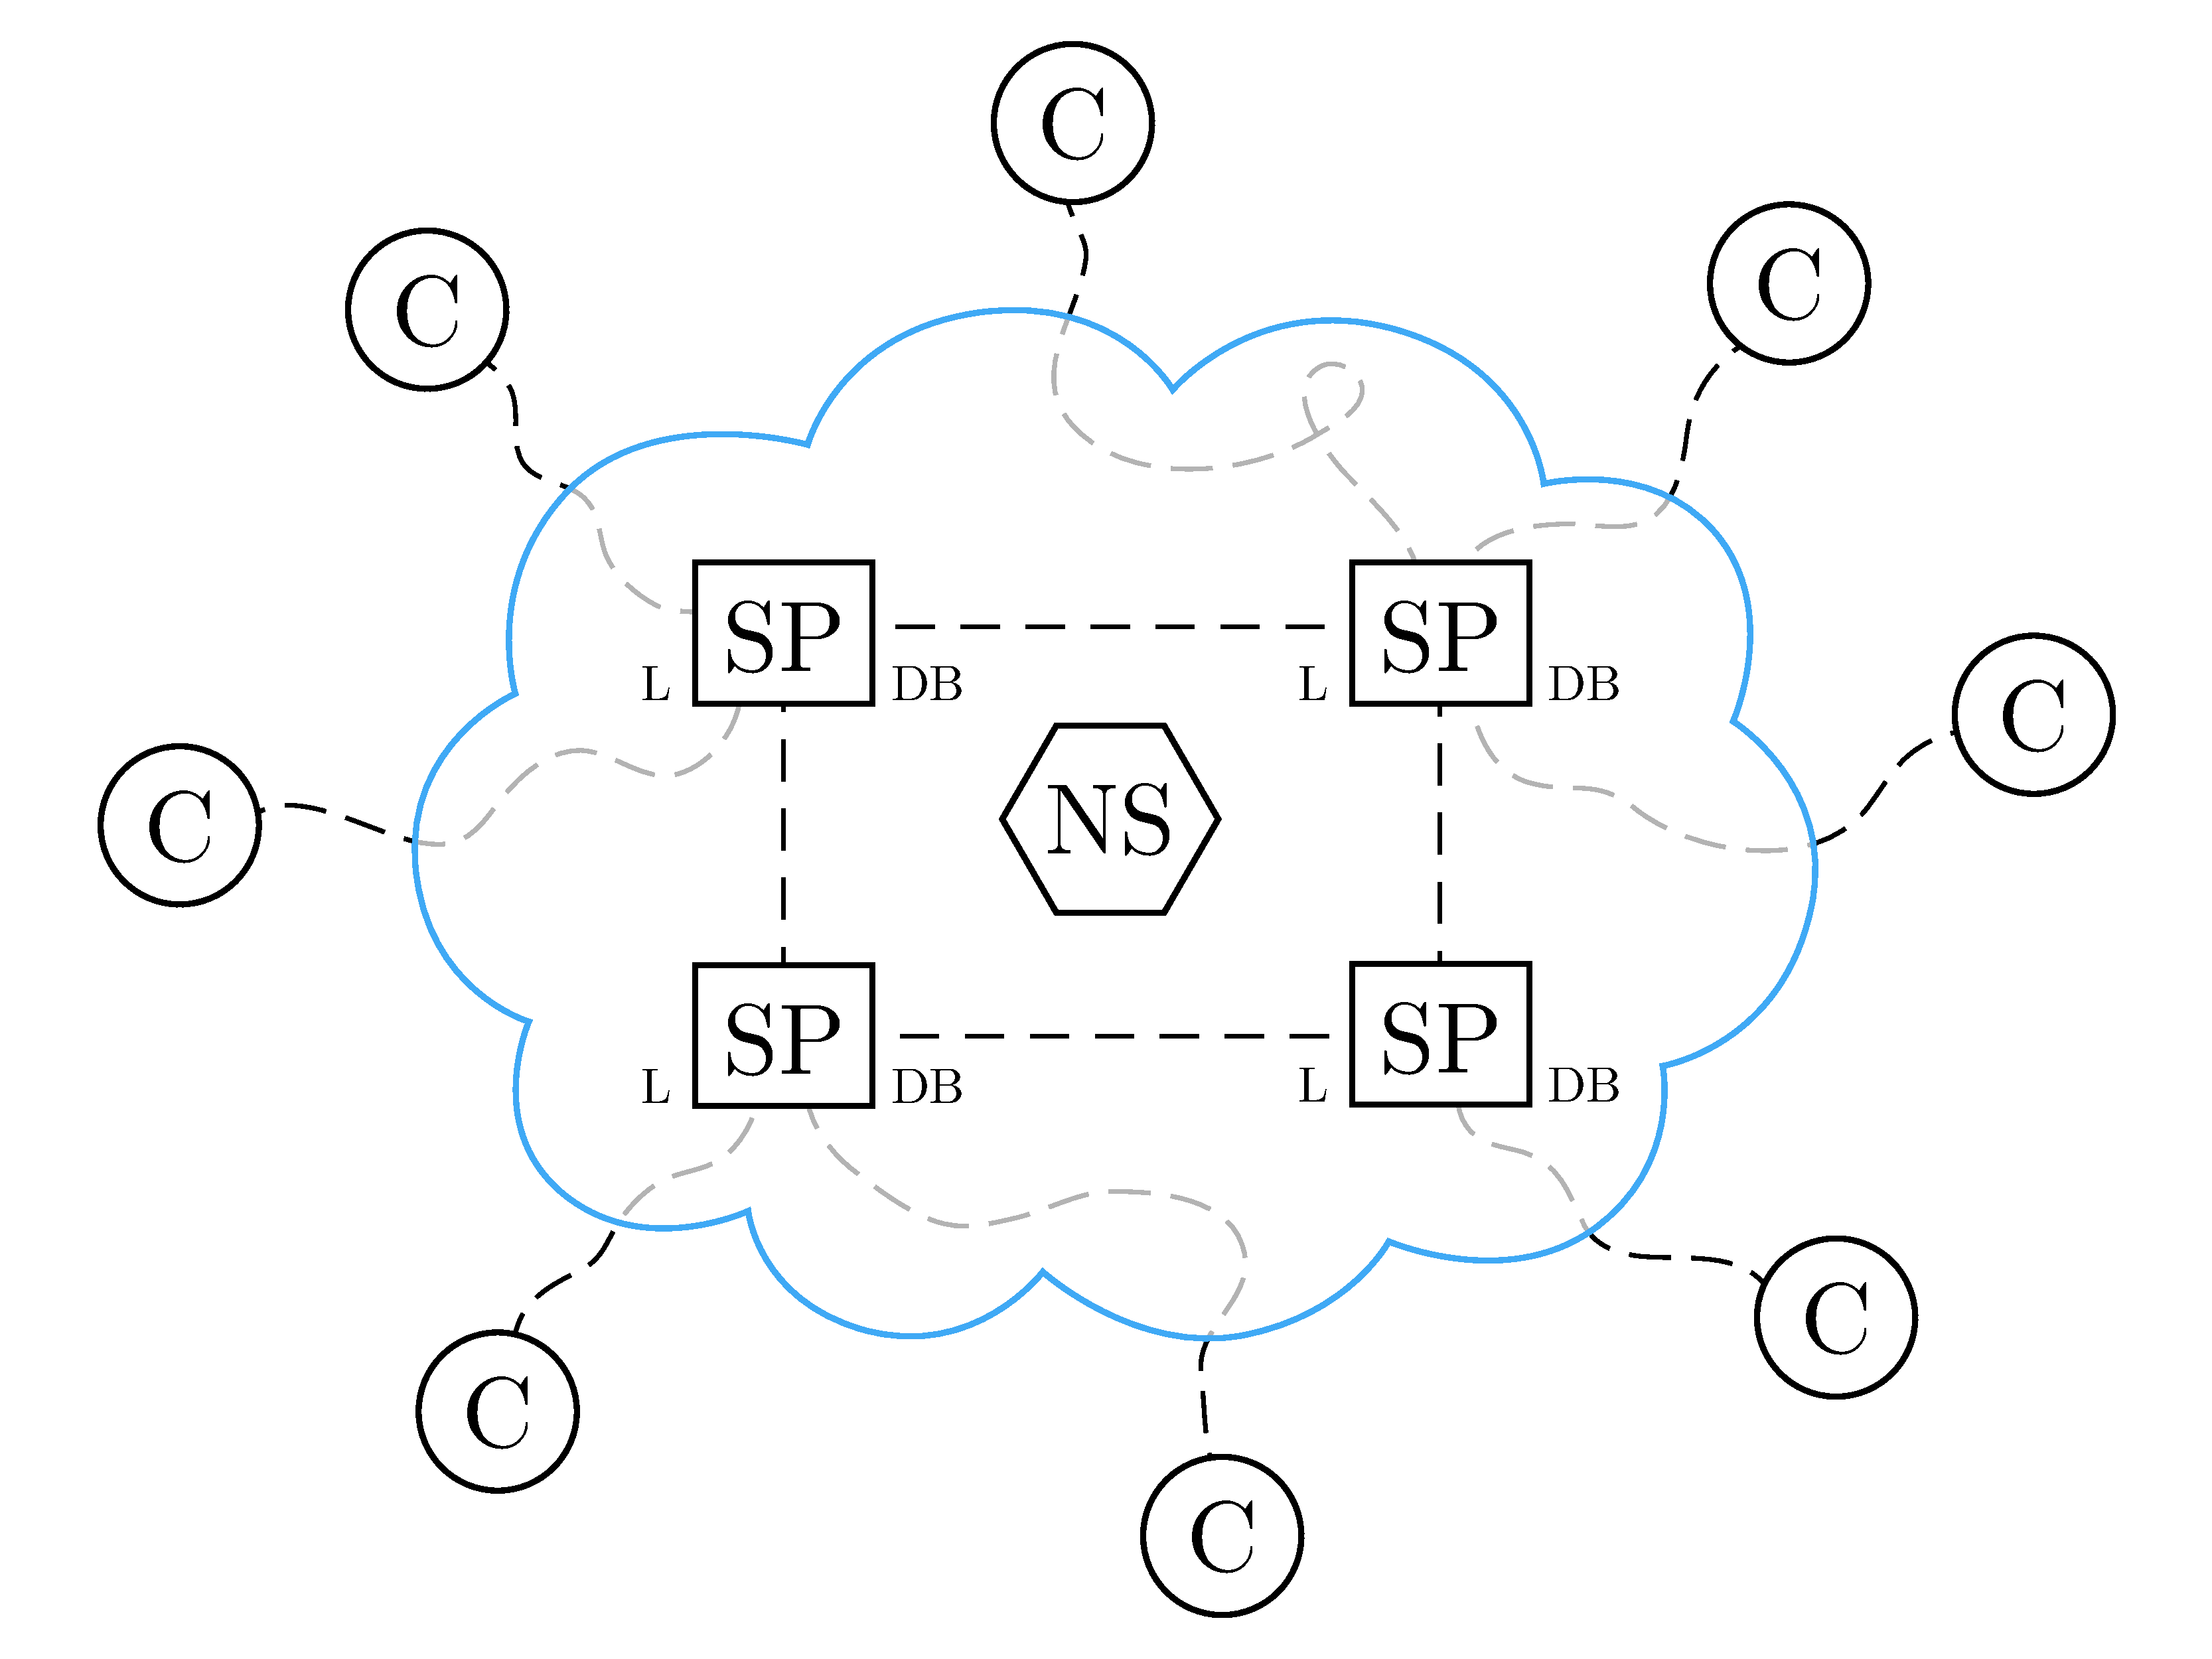
\includegraphics[width=0.8\textwidth]{include/assets/distributed-database.pdf}
  \caption{A distributed database with a number of servers/peers (SP) and a number of clients (C). Each server maintains a copy of the database (DB) protected by a distributed lock (L). The discovery process is facilitated by virtue of a name service (NS).}
  \flabel{distributed-database}
\end{figure}

Welcome to the course! Over six labs, from zero to five, you will learn and put
into practice the key components of a distributed system \cite{lecture1}. To
this end, you will implement your own distributed system, namely, a distributed
database of short messages known as fortunes \cite{fortune}.

The final configuration of the system that you will obtain by the end of the
fifth lab is depicted in \fref{distributed-database}. This system is composed of
a number of servers/peers (SP) and a number of clients (C). The servers maintain
copies of the database (DB) and ensure that these copies are kept consistent
across all the peers using a distributed locking mechanism (L). The clients
interact with this peer-to-peer network of servers in order to perform various
operations on the data. The participants of the network discover each other by
virtue of a so-called name service (NS); for clarity, these communications are
not shown.

In each lab, you will make a step towards the outlined goal by focusing on a
particular component of the final system:
\begin{enumerate}

  \setcounter{enumi}{-1}

  \item Standalone Database --- you will build a non-distributed database;

  \item Client-Server Database --- you will make your first attempt to
  distribute the database by considering the client-server model;

  \item Middleware: Object Request Brokers --- you will learn the importance of
  name services and implement a mechanism for interacting with them;

  \item Middleware: Peer-to-Peer Communications --- you will develop an
  algorithm for establishing and maintaining communications between peers who
  can arbitrary join and leave the system;

  \item Middleware: Distributed Locks --- you will implement mechanisms of
  distributed mutual exclusion to protect the data from concurrent operations;

  \item Client-Server Database with Replicas --- you will combine all the above
  components to produce a distributed database with data replication to ensure
  the efficiency and robustness of the overall system.

\end{enumerate}

For each lab, you will be given a skeleton of the code that corresponds to a
particular part of the system, and your task will be to understand what the code
does and to complete the implementation. The programming language that we shall
be using throughout the course is \python\ \cite{language}, more precisely, the
third version of \python\ \cite{python}. Even if you are not familiar with
\python, the language is straightforward to learn, and the source code, provided
to you, with a little bit of reading \cite{python-tutorial, python-library} will
be enough to readily get started and to successfully finish this programming
project. The above-mentioned skeletons for the labs and the corresponding
instructions (just like the one below for the zeroth lab) are provided to you on
the web page \cite{course} of the course.

\section{Introduction to the Lab}
\begin{figure}
  \centering
  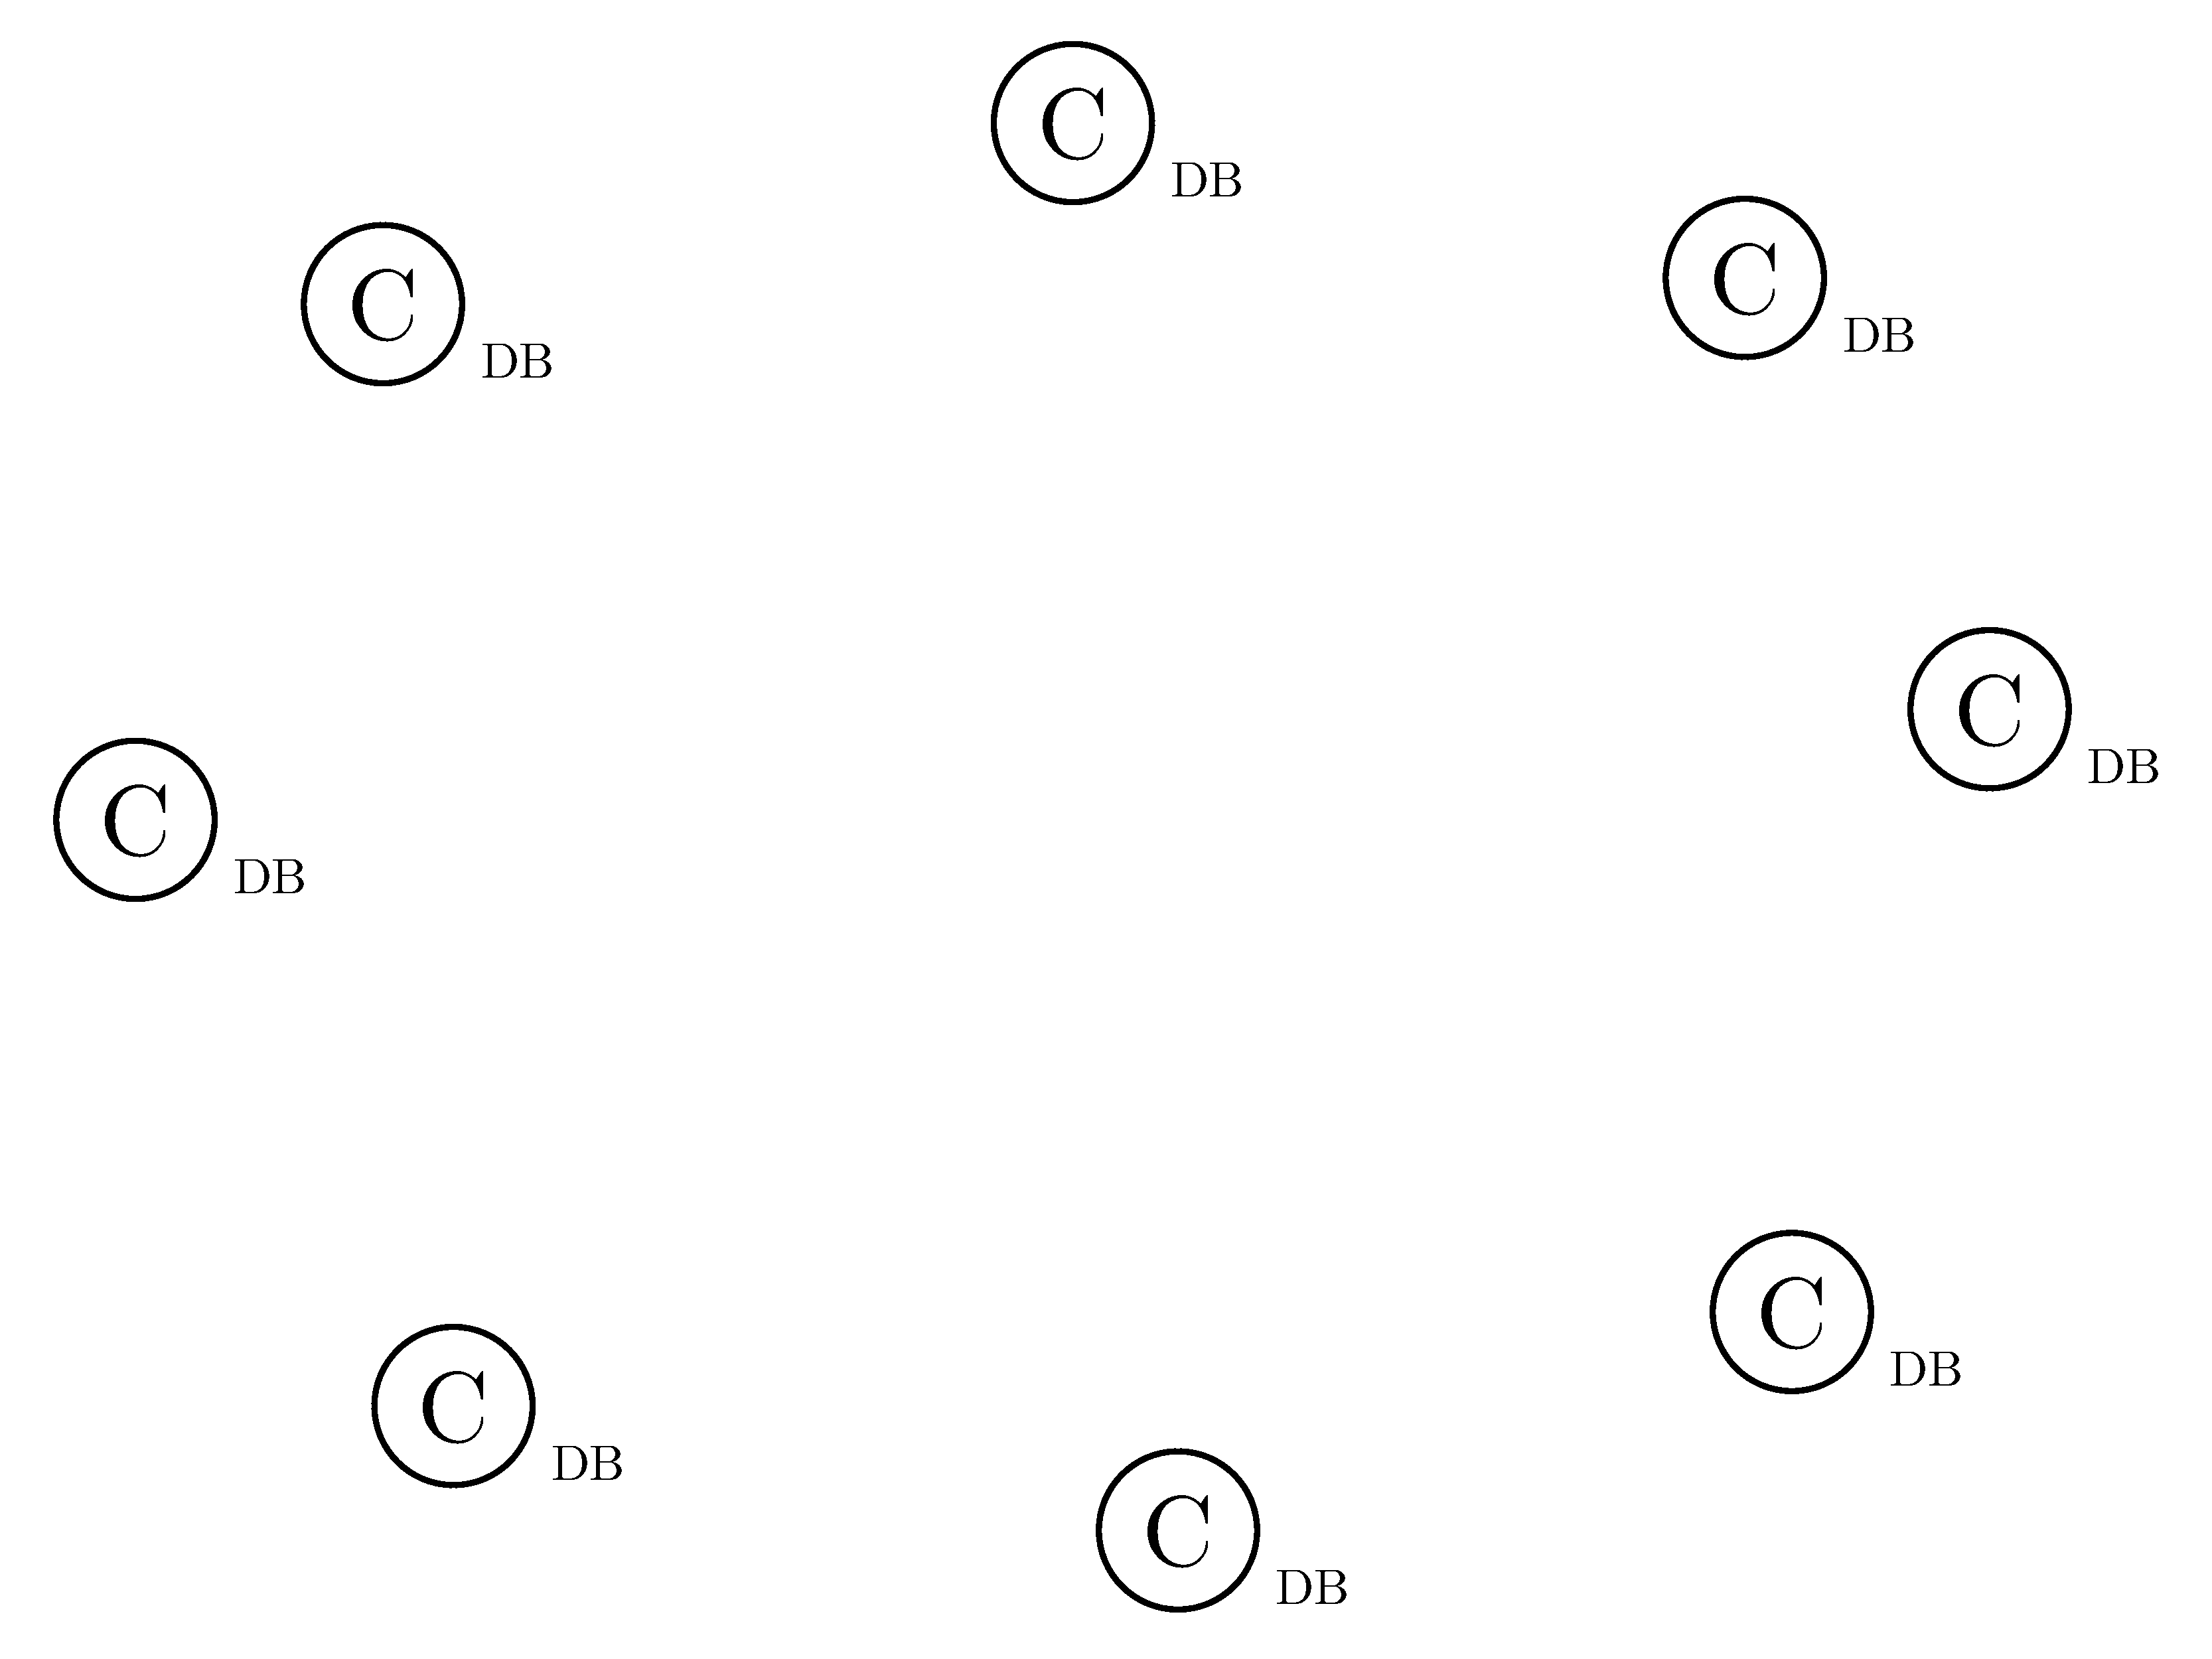
\includegraphics[width=0.8\textwidth]{include/assets/standalone-agents.pdf}
  \caption{A number of standalone clients (C) with their own databases (DB).}
  \flabel{standalone-agents}
\end{figure}

The goal of the zeroth lab is to introduce you to \python. Here we consider a
non-distributed system that consists of a number of standalone machines, each of
which acts as a server and as a single possible client of this server at the
same time. The scenario is depicted in \fref{standalone-agents}. The machines do
not interact with each other and perform all the operations on their own copies
of the data without any synchronization. In what follows, we shall refer to such
a standalone machine with the server/client functionality as simply
\classname{Client}.

\section{Data Format} \slab{data-format}
In all the labs, the list of fortunes, \ie, the actual data in our database,
will be stored in a text file conventionally called \filename{fortune.db}. Such
a file will be provided to you along with the source code; however, you are free
to come up with your own lists of fortunes. The format of \filename{fortune.db}
is rather straightforward: each message ends with a new line containing a single
percent sign (\texttt{\%}). For example, the following text contains two
fortunes:
\begin{fortune}
Everything should be made as simple as possible, but not simpler.
    -- Albert Einstein
%
According to the latest official figures, 43% of all statistics
are totally worthless.
%
\end{fortune}
Note that a message can have several lines, and there can be percent signs
inside of messages, which should be property taken into account when you start
writing your code for the interaction with the database.

\section{Your Task}
\subsection{Preparation} \slab{preparation}
Clone the repository of the programming project or download the latest snapshot
of the repository as a single zip archive \cite{repository}. The files relevant
to this lab are listed below; note that the paths are given with respect to the
\filename{src} directory of the repository. You should read and understand them.
\begin{itemize}

  \item \filename{lab0/client.py} --- the main file of the application that each
  machine of our non-distributed system is running (\leave);

  \item \filename{lab0/dbs/fortune.db} --- a list of fortunes (a thorough read
  and a deep understanding are not required here);

  \item \filename{modules/Server/database.py} --- a module with the
  \classname{Database} class needed for \filename{client.py} (\fix).

\end{itemize}

In order to run the application, open a terminal window, change the current
directory to \filename{lab0}, and execute the following command:\footnote{The
dollar sign (\texttt{\$}) will be used to denote a command prompt, and you
should not type this character in your terminal. Also, an alternative way to run
a \python\ script is to call \python\ explicitly. For example, you can try
running \texttt{python3 ./client.py -i}. Keep in mind that we use the third
version of \python.}

\begin{shell}
\$ ./client.py -i
\end{shell}
Following the menu of the program, you can try to read a random fortune from the
database or to compose a new one:
\begin{shell}
Choose one of the following commands:
    r            ::  read a random fortune from the database,
    w <FORTUNE>  ::  write a new fortune into the database,
    h            ::  print this menu,
    q            ::  exit the application.

Command> w Take it easy
Command> r
None
\end{shell}
As you can see, the issued commands do not work since the code is incomplete.
You can also open \filename{fortune.db} and observe that your new fortune is not
there.

\subsection{Implementation}
Your task is to fix the problem outlined in \sref{preparation}. Specifically,
you should complete the implementation of the following three function in
\filename{database.py}:
\begin{itemize}

  \item \code{\_\_init\_\_} --- initializes the database by parsing the content
  of \filename{fortune.db} and storing all found messages in an array (an
  instance variable);

  \item \code{read} --- returns a randomly chosen fortunes from the array (the
  \texttt{r} command in the application menu);

  \item \code{write} --- appends a new fortune to the array and updated
  \filename{fortunes.db} (the \texttt{w} command in the application menu).

\end{itemize}
Recall the note at the end of \sref{data-format}.

\section{Conclusion}
Having completed the lab, you can now perform the reading and writing operations
on the database. However, if you run several instances of the application on
different machines (see \fref{standalone-agents}) or in different terminal
windows on the same machine and try to add a new fortune in one of them, the
other clients will not see the change. The reason is that the clients do not
collaborate with each other and, therefore, do not try to keep their copies of
the data consistent. In the next lab, we will mitigate this problem.

\printbibliography

\end{document}
